\chapter{Specimen Thickness Through Off-Axis Electron Holography} \label{chap:appendix-specimen-thickness-off-axis-EH}
Contrary to CBED (\cref{chap:appendix-CBED}), the phase shift measured in off-axis EH is dependent on the whole specimen thickness $t_{\mathit{EH}}$ and can therefore be directly calculated through the measured phase shift (\cref{fig:pn-junction-thickness-off-axis-EH}):
\begin{equation}
  \label{eq:specimen-thickness-phase-shift}
  t_{\mathit{EH}} = \frac{\varphi_{\mathit{obj}}\left(\vb{r}\right)}{\sigma \phi_{\mathit{MIP}}\left(\vb{r}\right)},
\end{equation}
where $\sigma = \pi / \lambda E$ is an acceleration voltage dependent interaction constant and $\phi_{\mathit{MIP}}\left(\vb{r}\right)$ is the mean inner potential of the specimen \cite{Voelkl1999,Lehmann2002,Lichte2008}.
\begin{figure}[H]
  \centering
  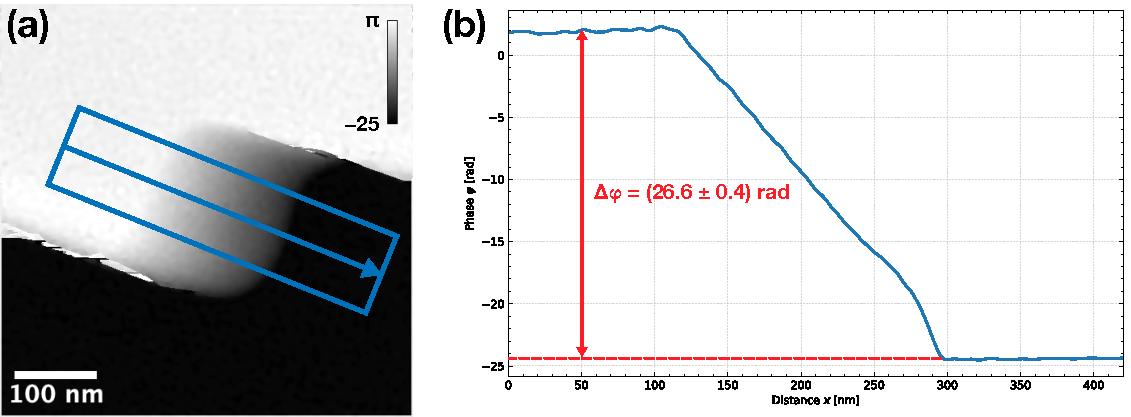
\includegraphics[width=\textwidth]{Figures/Specimen/pn-Junction/off-axis-EH-thickness.pdf}
  \caption{Determination of the specimen thickness $t_{\mathit{EH}}$ from off-axis EH with (a)~the reconstructed unwrapped phase $\varphi$ and (b) its corresponding line profile $\varphi\left(x\right)$. The specimen thickness is determined through the phase jump $\Delta \varphi = \SI{26.6 \pm 0.4}{rad}$ measured at the gradient of the specimen edge.}
  \label{fig:pn-junction-thickness-off-axis-EH}
\end{figure}
Using \cref{eq:specimen-thickness-phase-shift}, the measured phase jump of $\Delta \varphi = \SI{26.6 \pm 0.4}{rad}$ (where the measurement uncertainty is given by the standard deviation in the noise of the phase~$\varphi$), an interaction constant of $\sigma = \SI{6.53}{rad \per \volt \um}$ \cite{Beleggia2014} and a mean inner potential of $\phi_{\mathit{MIP}}\left(\vb{r}\right) = \SI{12.57}{\volt}$ for Si \cite{Kruse2006}, the specimen thickness is determined to be $t_{\mathit{EH}} = \SI{325 \pm 5}{\nm}$.
